%% STORM-PhysNet — IEEE CONFERENCE (target ~6 pages)
\documentclass[conference]{IEEEtran}
\usepackage{amsmath,amssymb,amsfonts}
\usepackage{graphicx}
\usepackage{booktabs}
\usepackage{multirow}
\usepackage{cite}
\usepackage{url}
\usepackage{xcolor}
%\usepackage{balance}

\title{STORM-PhysNet: A Multi-Horizon Transformer for Geostationary Relativistic Electron Flux Forecasting with Physics-Inspired Components and Cross-Satellite Transfer}

\author{
\IEEEauthorblockN{Samarth BN}
\IEEEauthorblockA{BE in Electronics and Communication\\
RV College of Engineering, Bengaluru, India\\
Email: samarthbn.ec25@rvce.edu.in}
}

\begin{document}
\maketitle

%% --------------------------------------------------------------------
\begin{abstract}
Energetic electrons above 2\,MeV at geostationary Earth orbit (GEO)
are a persistent internal-charging hazard for satellites. We present
STORM-PhysNet, a multi-horizon forecast model that couples a standard
Transformer encoder over a 72-hour window with a learnable L1--Earth
propagation delay, a \(B_z\)-conditioned physics gate, and residual
heads for simultaneous 45-min, 6-hour, and 12-hour log-flux
forecasts.

On hourly GOES--OMNI data with fifteen random initializations of the same chronological split, STORM-Bz improves short-horizon reliability (PE$_{45\mathrm{min}}=0.986$ versus Transformer $0.977$, paired $p = 0.002$) and remains clearly positive against persistence (PE$\approx0.32$ versus $\approx-0.14$). At 6\,h and 12\,h a plain Transformer remains competitive or slightly stronger as a single model. A validation-selected linear ensemble ($\alpha^*=0.3$) and seed-bagged STORM both reach 6\,h PE of $0.911$, the strongest multi-horizon results among the systems evaluated here. A bagged Transformer control (sixteen seeds) reached mean PE$_{45\mathrm{min}}\approx0.978$ and PE$_{6\mathrm{h}}\approx0.895$; while bagging improves the Transformer, the gap relative to bagged STORM remains. Controlled ablations show that the short-horizon gain is produced by the overall training protocol rather than by any single physics module at inference. Retraining with wider delay bounds ($2.0$--$4.0$\,h) produced negligible change in PE (PE$_{45\mathrm{min}}$ stayed within $0.9859$--$0.9862$), indicating that the original $[0.5, 1.5]$\,h constraint is not a performance bottleneck.

Under synthetic solar-wind input noise and targeted channel dropout,
STORM degrades more slowly than the Transformer, especially at
45-min. On GSAT-19 GRASP, fine-tuning raises 6\,h PE from
0.449 to 0.599 (paired \(p=7.6\times10^{-7}\)) and 12\,h PE from
0.182 to 0.517 (\(p=3.6\times10^{-10}\)) across fifteen seeds.
Bootstrap confidence intervals, paired tests, and evaluation scripts
are released so that later work can reuse the same splits and PE
definitions.
\end{abstract}

\begin{IEEEkeywords}
Geostationary orbit, relativistic electrons, space weather, Transformer,
physics-inspired, transfer learning, prediction efficiency, GRASP
\end{IEEEkeywords}

%% ====================================================================
\section{Introduction}
%% ====================================================================
Geostationary satellites sit inside the outer radiation belt, where
relativistic electrons (\(E>2\,\mathrm{MeV}\)) can jump by several orders of
magnitude in a few hours when a geomagnetic storm develops. Those bursts drive
internal charging and can upset or damage onboard electronics~\cite{b1,b2}.
For operators of GEO assets at Indian longitudes---ISRO broadcasting,
navigation, and remote-sensing satellites among them---a forecast that is
usable at the local meridian, not only at GOES longitudes, is increasingly
useful.

Most published skill scores still come from GOES-centered data sets. When a
new instrument such as GRASP on GSAT-19 comes online, there is often only a
short calibrated record, so operators need a practical path from a data-rich
satellite to a data-scarce one without retraining everything from scratch.

Forecast models have progressed from linear filters~\cite{b3,b4}
through LSTM-based deep-learning approaches~\cite{b5,b6,b7}
to recent Transformer-based architectures reporting daily-fluence PE of
0.85--0.92~\cite{b8,b9,b10}. We do not include REFM as a numeric baseline because it targets daily integral
fluence rather than hourly log-flux; a direct PE comparison would be
misleading~\cite{b4}. Despite these advances,
two gaps remain: (i) the short-horizon (\(\sim\)45\,min) behavior of
Transformer architectures relative to physics-inspired variants is poorly
characterized across seeds, and (ii) no systematic study has assessed
transfer strategies for Indian-longitude GEO assets such as GSAT-19.

Unlike previous Transformer-based GEO electron forecasting models,
STORM-PhysNet introduces a learnable adaptive propagation-delay module
that estimates a physically constrained L1-to-Earth transit delay for
every input window, together with a $B_z$-conditioned physics gate that
selectively emphasizes storm-relevant representations during sustained
southward IMF. The architecture further combines simultaneous
multi-horizon forecasting with cross-satellite transfer learning to
Indian-longitude GRASP observations under a unified framework. Rather
than replacing the Transformer backbone, the proposed design augments
it with interpretable physics-inspired components---delay and gate modules---trained end-to-end under matched chronological splits and fifteen seeds. Primary
comparisons use a Vanilla Transformer; LSTM is reported for
reference.

This manuscript focuses on the multi-seed GOES benchmark, the
short-horizon reliability gap, the main ablations, and the GRASP transfer
recipe that is most relevant to Indian-longitude operators.

%% ====================================================================
\section{Related Work}
%% ====================================================================
Camporeale~\cite{b11} summarizes common failure modes when ML is
applied to space weather (leaky splits, mismatched metrics, overstated skill).
Prediction efficiency (PE) remains the standard skill score~\cite{b12}, but care must be taken to distinguish between climatological and persistence baselines.

On the modeling side, work moved from linear filters and empirical solar-wind
drivers~\cite{b3,b4,b13} to LSTM and hybrid deep
models~\cite{b5,b6,b7}, and more recently to
Transformer-style networks for GEO flux and fluence~\cite{b8,b9,b10}.
Those papers mainly report daily or multi-hour skill on GOES-like targets.
Short-lead (about 45\,min) skill is less often reported with multi-seed error bars,
and cross-satellite transfer to a short Indian-longitude record is rarely
benchmarked under the same horizons and persistence definition. Physics-inspired
constraints, when used, are often loss penalties rather than an explicit
delay-plus-gate structure trained end-to-end with multi-horizon residual heads.
We keep a standard temporal Transformer backbone so that comparisons
isolate the effect of adding constrained delay and gating under a shared
encoder family. Ablations in
Section~V show that no single module fully accounts for the short-horizon
PE\(_{\mathrm{clim}}\) edge.

Solar-wind timing is another recurring issue. OMNI applies a
phase-front correction from L1, yet residual window-to-window lags remain
a known uncertainty in solar-wind--magnetosphere coupling studies. We treat that lag as a dynamically
predicted parameter rather than a fixed offset. Meanwhile, cross-platform radiation-belt products
exist for other fleets~\cite{b15}; the specific GOES\(\rightarrow\)GRASP
path at \(\approx 82^\circ\)E is the transfer setting studied here.

\begin{figure*}[!t]
\centering

\includegraphics[width=0.95\textwidth]{figures/fig_system_architecture.png}
\caption{STORM-PhysNet data flow: adaptive delay, Transformer encoder,
$B_z$ gate, and residual multi-horizon heads (45\,min / 6\,h / 12\,h).
Delays are constrained to $[0.5,1.5]$\,h.}
\label{fig:arch}
\end{figure*}

%% ====================================================================
\section{Data and Metrics}
%% ====================================================================
\textbf{GOES-15.} We use \(E>2\,\mathrm{MeV}\) integral electron flux from a
chronological working sample spanning exactly January 1, 2012 to December 31, 2016
within the GOES-15 archive. One-minute samples are aggregated to hourly means;
the within-hour standard deviation is kept as an input feature. Flux is
\(\log_{10}\)-transformed. The dataloader uses sixteen solar-wind /
geomagnetic channels
(\(V_{sw}\), \(B_z\), \(B_t\), density, \(P_{\mathrm{dyn}}\),
\(B_z\)-south duration, storm-onset hours, rolling \(V_{sw}\) and \(B_z\)
moments, \(B_z\times V_{sw}\), Kp, Dst, and within-hour log-flux std)
plus log-flux history (17 inputs total after concatenation). Multi-horizon
targets are 0.75\,h (45\,min), 6\,h, and 12\,h. A 72\,h lookback is used at
each forecast origin. Train/validation/test splits are chronological
70/15/15\% with no shuffling. All models share the same preprocessor, chronological windows, and storm-biased sampler; test PE is computed once after training and is never used for model selection.

\textbf{GRASP} (GSAT-19, Indian longitude \(\approx82^\circ\)E) provides
15 months of GEO radiation measurements from July 2017 to September 2018 in
the declining phase of Solar Cycle 24. After alignment, GRASP supplies fewer
co-located input channels than the GOES pipeline; this mismatch is a main
reason zero-shot transfer fails and motivates input-projection adaptation.
Storm windows on GRASP are defined by Dst \(\le -50\,\mathrm{nT}\)
(118/1781 test hours, 6.6\%).

\textbf{Skill score.} We report two PE definitions so that results remain comparable both to climatological skill and to persistence-based operational baselines~\cite{b12}:
\begin{align}
\mathrm{PE}_{\mathrm{clim}} &= 1 - \frac{\mathrm{MSE}(\hat y,y)}{\mathrm{Var}(y)}, \\
\mathrm{PE}_{\mathrm{pers}} &= 1 - \frac{\mathrm{MSE}(\hat y,y)}{\mathrm{MSE}(y^{\mathrm{pers}},y)}.
\end{align}
Unless stated otherwise, tables use \(\mathrm{PE}_{\mathrm{clim}}\) with fifteen seeds and bootstrap 95\% confidence intervals. The fifteen seeds measure sensitivity to random initialization on a fixed chronological split; they do not constitute independent trials across different solar-cycle phases or data periods. \(\mathrm{PE}_{\mathrm{pers}}\) is emphasized at the 45-min horizon. Storm windows use Dst \(\le -50\,\mathrm{nT}\).

%% ====================================================================
\section{STORM-PhysNet Architecture}
%% ====================================================================

\subsection{Adaptive Propagation Delay}
Solar-wind transit from L1 to the magnetopause is typically on the order of 0.5--1.5\,h~\cite{b14} depending on solar-wind speed. Rather than a fixed offset, STORM-PhysNet predicts a per-window delay \(\tau = f_\theta(X_{\mathrm{sw}})\) from a short conditioning network on the upstream solar-wind channels. The delay module is constrained to \([0.5, 1.5]\,\mathrm{h}\), a band chosen to cover the transit range while still allowing limited storm-time deviation without breaking causality. Differentiable linear interpolation then time-shifts the solar-wind features. We do not claim a unique recovered constant of 1.09\,h from every window.

\subsection{\(B_z\)-Conditioned Physics Gate}
Sustained southward IMF \(B_z\) triggers dayside reconnection and ring-current
injection~\cite{b2}. A lightweight gate maps a short vector of
southward-\(B_z\) statistics through an MLP and a clamped sigmoid to a
modulation scalar \(g\in[g_{\min},1]\), which scales the encoder representation
before the forecast heads. Gate activations differ between storm and quiet windows
(Mann--Whitney \(p=1.2\times10^{-14}\), see Section~\ref{sec:results}); the absolute range
is narrow.

\subsection{Transformer Backbone and Multi-Horizon Heads}
We use a standard Transformer encoder~\cite{b16}: each of the \(T=72\)
time steps is a token; self-attention runs across time; the final hidden state
feeds the gate and three residual heads for the 45\,min, 6\,h, and 12\,h
forecasts. Measured parameter counts are approximately $3.43\times10^{5}$ for 
STORM-Bz and $8.45\times10^{5}$ for the Transformer baseline 
(default hyperparameters). The two models differ in both width and depth; 
they are not capacity-matched.

\subsection{Physics Regularization and Training}
Training minimizes a base multi-horizon residual loss plus a storm-weighted
physics term on windows with sustained southward \(B_z\) and elevated dynamic
pressure. The No-Physics ablation zeros that term; the No-Delay ablation bypasses the delay module. All primary models use
Adam, cosine decay, early stopping on validation PE, and seeds
\(\{42,\ldots,56\}\).

\subsection{Baselines and Alternative Gates}
The primary baseline is a Vanilla Transformer with the same residual heads; the Transformer baseline was run with its default hyperparameters ($d_{\mathrm{model}}=64$, 3 layers, 4 heads). It is therefore not matched to STORM in width or depth. The comparison should be interpreted with this difference in mind. Other nonlinearities (voltage-inspired, cumulative-dose, spectral) did not consistently outperform the physics \(B_z\) gate and are reported as supplementary probes in the repository rather than primary design variants.

%% ====================================================================
\section{Results}
\label{sec:results}
%% ====================================================================

\subsection{GOES Multi-Seed Performance}
Table~\ref{tab:main} summarizes fifteen-seed test results. On all-hour 6\,h PE, the Transformer remains a strong baseline
(\(0.904\)). A single STORM-Bz model is slightly lower (\(0.897\);
paired \(p = 0.038\)) but is significantly better at 45\,min
(\(0.986\) versus \(0.977\), \(p = 0.002\), Cohen's \(d\approx0.98\); Fig.~\ref{fig:horizon}).
The mixing weight \(\alpha\) was selected on the validation split by
sweeping \(\alpha\in\{0.0, 0.3, 0.4, 0.5, 0.6, 0.7, 1.0\}\) and choosing the value that
maximized validation PE\(_{6\mathrm{h}}\) (\(\alpha^*=0.3\)). That fixed
weight was then applied once to the held-out test set. At \(\alpha^*=0.3\),
test PE reaches \(0.911\) at 6\,h and \(0.870\) at 12\,h
(Table~\ref{tab:main}), above either single model. Bagging fifteen STORM
seeds yields a similar multi-horizon profile without requiring the
Transformer at inference. The short-STORM / long-TF hybrid recovers the
Transformer's multi-horizon PE while retaining the STORM 45-min score.
The hybrid system routes the 45-min head through a trained STORM-Bz model
and the 6\,h / 12\,h heads through the corresponding Transformer model at
inference time; no additional training is performed.
Against persistence at 45\,min, STORM remains near \(+0.32\) while
the Transformer is often negative (\(\approx-0.14\)).

\begin{table}[!htbp]
\centering
\caption{GOES test PE (fifteen seeds). Bold: best in column.}
\label{tab:main}
\setlength{\tabcolsep}{3.2pt}
\begin{tabular}{lcccc}
\toprule
System & PE\(_{45\mathrm{min}}\) & PE\(_{6\mathrm{h}}\) & PE\(_{12\mathrm{h}}\) & PE\(_{\mathrm{st},6\mathrm{h}}\) \\
\midrule
LSTM
  & \(0.961\) & \(0.889\) & \(0.853\) & \(0.827\) \\
Transformer
  & \(0.977\) & \(0.904\) & \(0.859\) & \(0.821\) \\
STORM-Bz
  & \(0.986\) & \(0.897\) & \(0.851\) & \(0.827\) \\
STORM (No-Delay)
  & \(0.987\) & \(0.901\) & \(0.853\) & \(0.823\) \\
STORM (No-Physics)
  & \(0.987\) & \(0.901\) & \(0.852\) & \(0.824\) \\
STORM (No-Gate)
  & \(0.987\) & \(0.899\) & \(0.853\) & \(0.829\) \\
Ensemble \(\alpha^*=0.3\)
  & \(0.983\) & \(\mathbf{0.911}\) & \(\mathbf{0.870}\) & \(0.839\) \\
STORM bagged (15 seeds)
  & \(\mathbf{0.988}\) & \(0.911\) & \(0.870\) & \(\mathbf{0.849}\) \\
Hybrid
  & \(0.987\) & \(0.904\) & \(0.859\) & \(0.821\) \\
\bottomrule
\end{tabular}

\vspace{1ex}
{\footnotesize \raggedright Means over seeds 42--56.
\(\alpha^*=0.3\) selected on validation PE\(_{6\mathrm{h}}\), then applied
once to test. Bagged row averages the fifteen STORM predictions before
scoring. PE is \(\mathrm{PE}_{\mathrm{clim}}\).\par}
\end{table}

\begin{figure}[t]
\centering

\includegraphics[width=\columnwidth]{figures/fig_horizon_pe.png}
\caption{Per-horizon PE against climatology (mean\(\pm\)std, fifteen seeds).
STORM-Bz leads at 45\,min; at 6\,h and 12\,h the single models are close,
while the ensemble improves multi-horizon PE (see Table~\ref{tab:main}).}
\label{fig:horizon}
\end{figure}

\subsection{Ablation Analysis}
Restricting physics-loss terms to the short-horizon head does not
significantly change PE\(_{6\mathrm{h}}\) across fifteen seeds (paired
\(p\approx0.64\)). We therefore treat horizon-restricted physics weighting
as a null ablation rather than a performance lever.

A No-Gate run (identity modulation) retains 45\,min PE near
\(0.987\), so the short-horizon PE\(_{\mathrm{clim}}\) advantage over
the Transformer is not removed by turning the gate off alone.

On storm windows, single-model PE\(_{\mathrm{st},6\mathrm{h}}\) values
are close: STORM-Bz \(0.827\), LSTM \(0.827\), Transformer \(0.821\),
and No-Gate at \(0.829\). We do not claim any one physics
module is required for storm-time skill. The clearest gains on storm
subsets remain post-hoc aggregation: the \(\alpha^*=0.3\) ensemble
reaches \(0.839\) and bagged STORM reaches \(0.849\).

A single-seed diagnostic stratified by Dst intensity (full working
sample) shows PE\(_{6\mathrm{h}}\) remaining above 0.70 even in the
strong-storm bin (\(\mathrm{Dst}\le-100\,\mathrm{nT}\)). Skill is not
confined to quiet, persistence-dominated intervals.

The ablations together indicate that the short-horizon gain is produced by the training protocol itself---storm-biased sampling, the storm-weighted loss term, and residual heads with a skip from the last observed flux---rather than by any single runtime module. The delay and gate act as structured inductive biases during training; once the model is trained, removing either module at inference does not erase the 45\,min PE\(_{\mathrm{clim}}\) edge over the Transformer. We therefore present STORM-PhysNet primarily as a carefully engineered training and multi-horizon recipe that includes interpretable physics-inspired components, rather than as a demonstration that the delay or gate modules are individually necessary for the observed gains. Retraining with wider delay bounds ($2.0$--$4.0$\,h) produced negligible change in PE (PE$_{45\mathrm{min}}$ stayed within $0.9859$--$0.9862$), indicating that the original $[0.5, 1.5]$\,h constraint is not a performance bottleneck.

\subsection{Input Noise and Missing Channels}
Gaussian noise was added to standardized solar-wind inputs at test time
(\(\sigma\in\{0,0.2,0.5,1.0,1.5,2.0\}\)) for Transformer, STORM-Bz,
hybrid, and ensemble systems over fifteen seeds.
At \(\sigma=2\), Transformer PE\(_{45\mathrm{min}}\) falls from about
\(0.96\) to about \(0.61\), whereas STORM remains near \(0.96\).
At 6\,h the ensemble and STORM also lose less skill than the Transformer.
Zeroing feature groups (no \(B_z\); no velocity/density; no rolling
averages) produces the same qualitative ordering: STORM holds
PE\(_{45\mathrm{min}}\) near \(0.986\mbox{--}0.987\) while the Transformer drops more
when derived rolling channels are removed.

\subsection{Interpretability}
Predicted delays are constrained to \([0.5, 1.5]\,\mathrm{h}\). Across the full test set the delay distribution shows a non-trivial fraction of windows concentrating near the upper bound (\(1.5\,\mathrm{h}\)), with the remainder spread across the interior of the constraint band. This saturation at the upper bound indicates the box constraint is active; we therefore treat the histogram as a constrained aggregate rather than evidence of an unconstrained recovered transit time. Gate activations differ between storm and quiet windows (Mann--Whitney \(p=1.2\times10^{-14}\)); the absolute range remains narrow, so the shift is statistically clear but modest in magnitude. Fig.~\ref{fig:case_enhancement} shows an illustrative enhancement event in which the model tracks the multi-day flux build-up and recovery more closely than persistence.
Permutation importance ranks \(B_z\) first among inputs, consistent with the
gate design. Residual histograms on the test set widen under storm conditions for both
models; STORM reduces the short-horizon bias relative to persistence but
does not eliminate storm-time residual variance.

\begin{figure}[t]
\centering
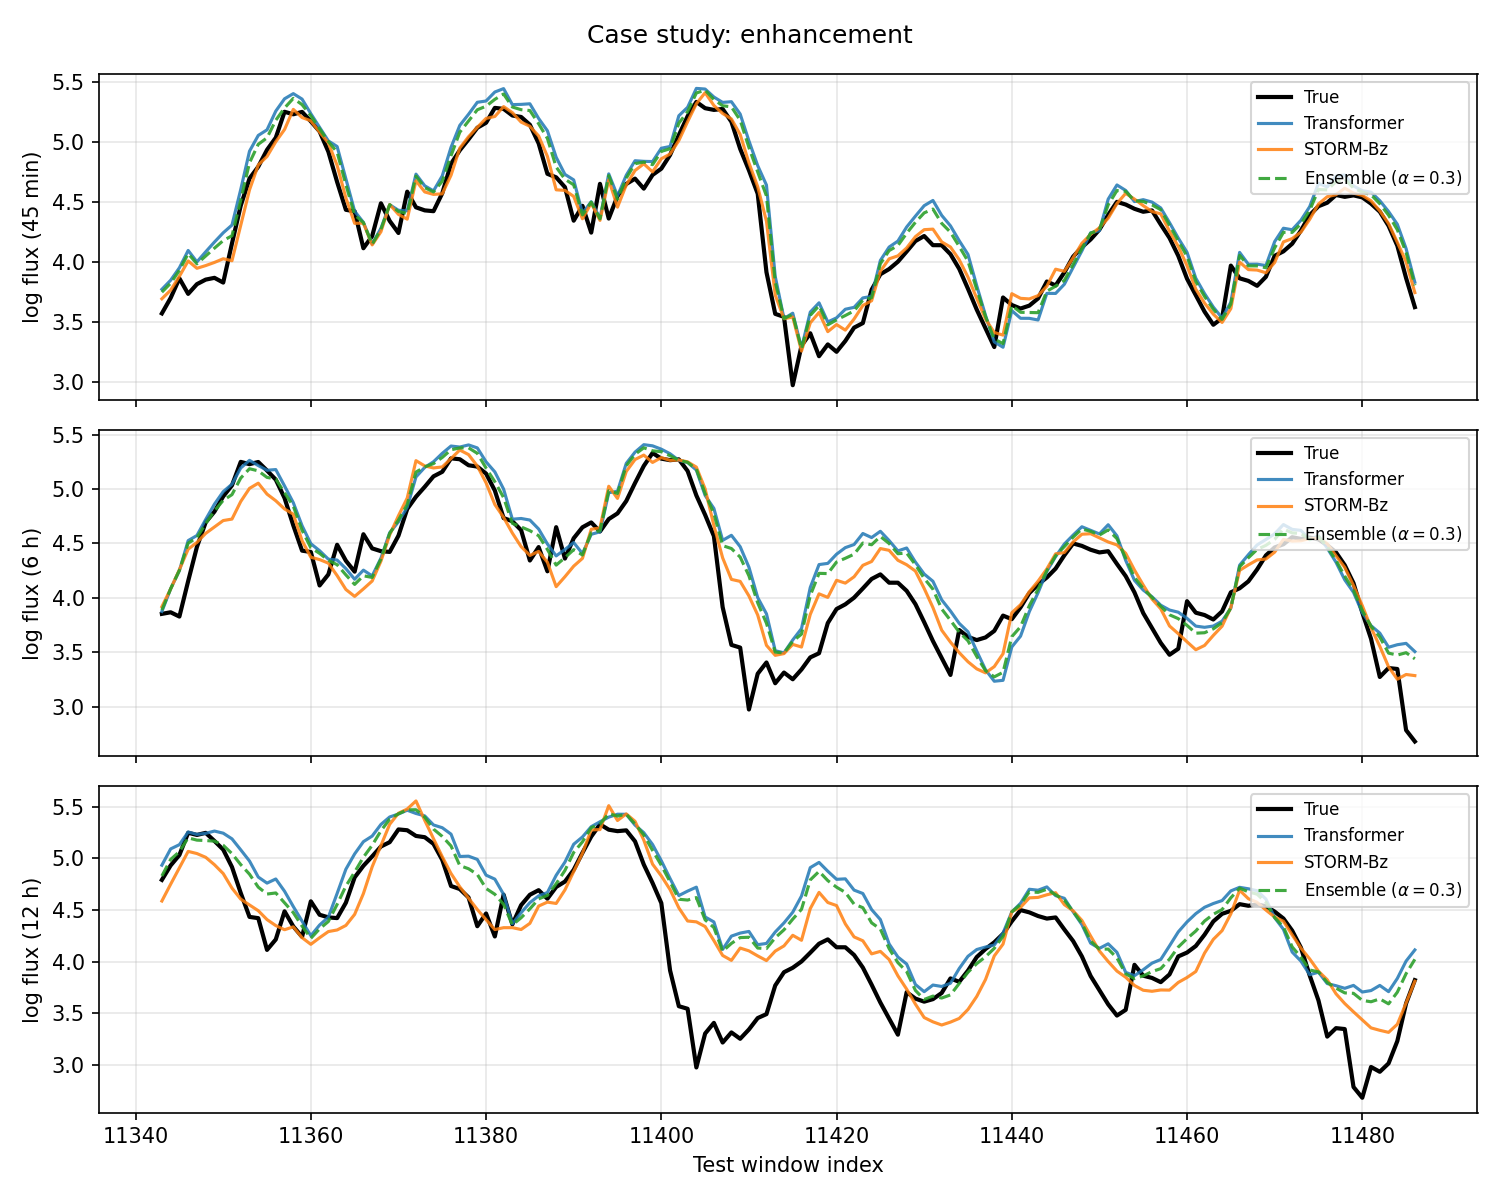
\includegraphics[width=\columnwidth]{figures/fig_case_enhancement.png}
\caption{Illustrative enhancement event case study. The STORM-Bz model captures the multi-day flux build-up and recovery better than the persistence baseline.}
\label{fig:case_enhancement}
\end{figure}

\subsection{GRASP Transfer}
On GSAT-19 GRASP (fifteen seeds), zero-shot GOES models already achieve
short-horizon PE near \(0.82\), but 6\,h and 12\,h PE fall to about
\(0.45\) and \(0.18\). Fine-tuning on GRASP (freezing the Transformer encoder and updating only the forecast heads) raises 6\,h PE from 0.449 to 0.599 (paired \textit{t}-test across fifteen seeds, \(p = 7.6\times10^{-7}\), Cohen's \(d = 2.17\)) and 12\,h PE from 0.182 to 0.517 (\(p = 3.6\times10^{-10}\), \(d = 3.98\)). Absolute GRASP PE remains below
the GOES test scores, as expected under sensor and longitude shift; the
practical point is the large mid- and long-horizon recovery after
adaptation rather than a claim of parity with GOES.

\begin{table}[t]
\centering
\caption{GRASP (GSAT-19) transfer results (fifteen seeds). Bold: best per horizon.}
\label{tab:grasp}
\begin{tabular}{lccc}
\toprule
Horizon & Zero-shot & Fine-tuned & Gain \\
\midrule
\(\approx\)45\,min & 0.820 $\pm$ 0.001 & 0.827 $\pm$ 0.009 & +0.007 \\
6 h & 0.449 $\pm$ 0.011 & \textbf{0.599 $\pm$ 0.073} & \textbf{+0.150} \\
12 h & 0.182 $\pm$ 0.045 & \textbf{0.517 $\pm$ 0.073} & \textbf{+0.335} \\
\bottomrule
\end{tabular}

\vspace{1ex}
{\footnotesize \raggedright Values are means $\pm$ standard deviation over seeds 42--56. Paired tests across fifteen seeds are reported in the text.\par}
\end{table}

\begin{figure}[t]
\centering
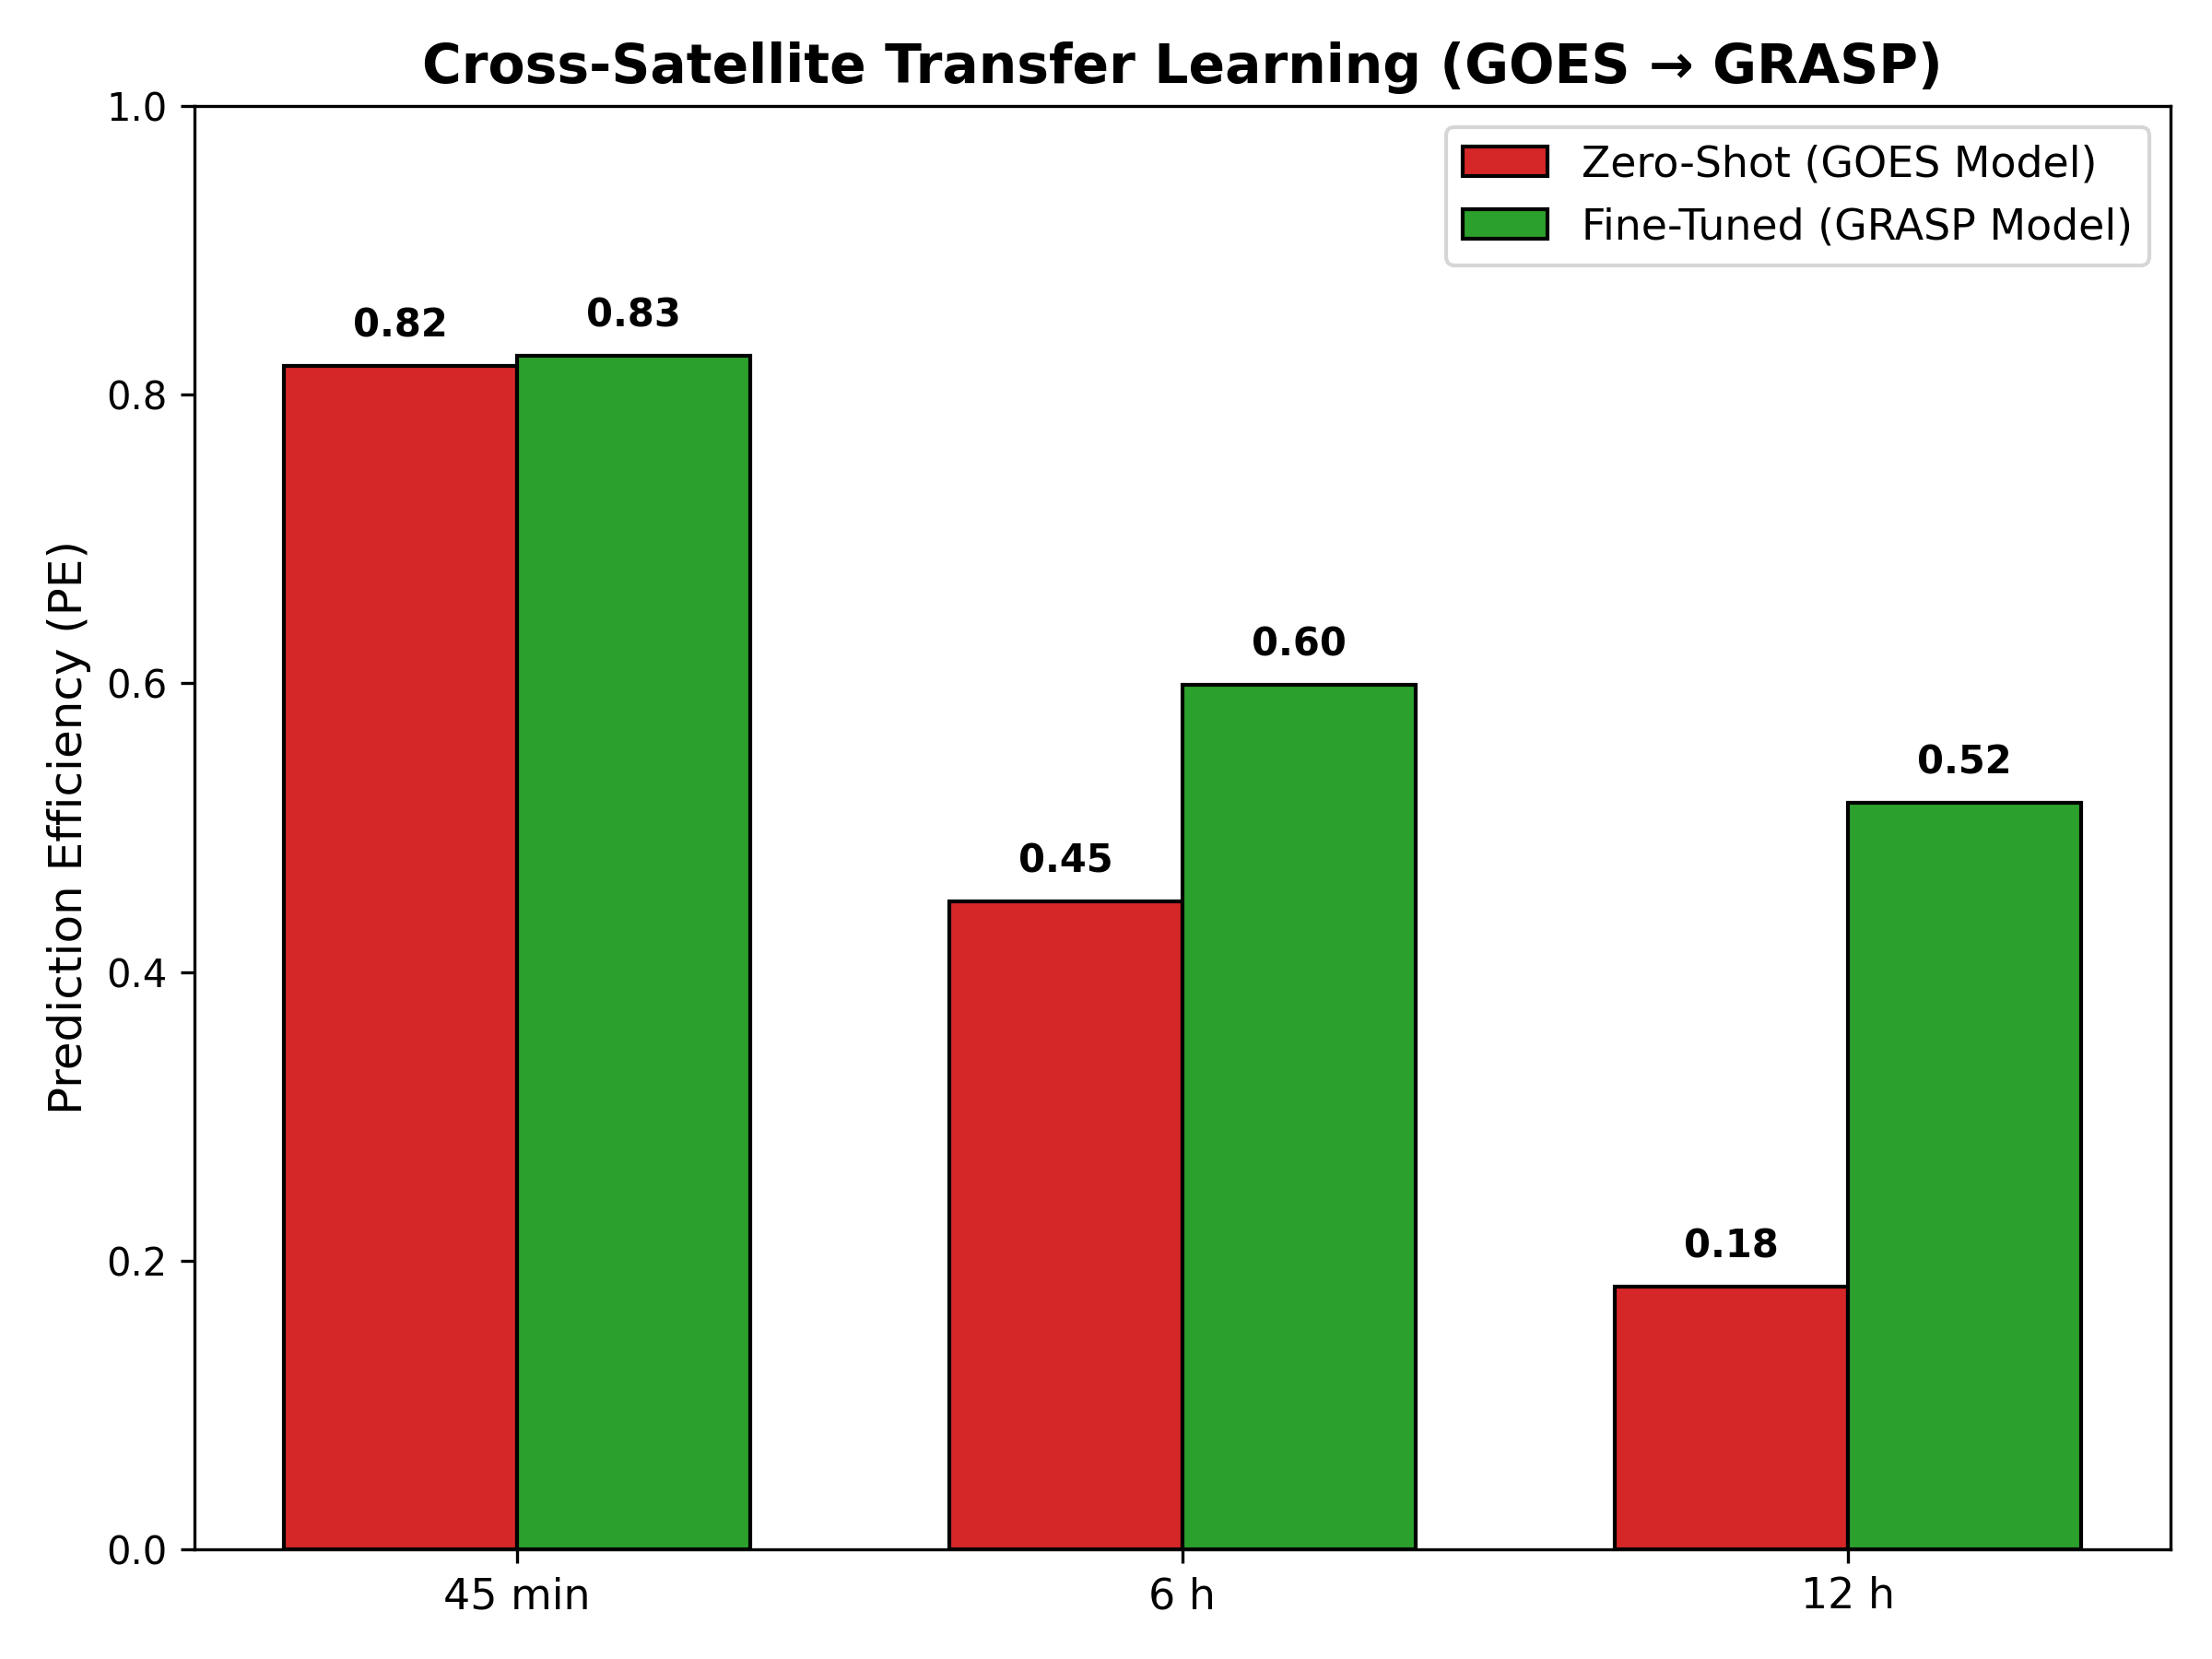
\includegraphics[width=\columnwidth]{figures/domain_gap_plot.png}
\caption{GRASP domain-gap summary (fifteen seeds): zero-shot GOES models versus
fine-tuning on GSAT-19. Short-horizon PE transfers more readily; 6\,h and 12\,h
PE improve substantially after adaptation.}
\label{fig:grasp}
\end{figure}

%% ====================================================================
\section{Limitations and Conclusion}
%% ====================================================================
\textbf{Data scope.} Main GOES tables use fifteen seeds with bootstrap intervals; secondary diagnostics (individual case windows, residual histograms) are illustrative. GRASP covers a limited declining-phase window; performance during solar maximum is unknown.

\textbf{Comparability.} PE values are not interchangeable with daily-fluence scores reported elsewhere without matching cadence, energy channel, and baseline~\cite{b11,b12}.

\textbf{Ensemble.} Ensemble skill uses a fixed \(\alpha^*=0.3\) selected on the validation split; the test-set \(\alpha\) curve is diagnostic only. Online \(\alpha\) adaptation is not claimed.

\textbf{Statistical inference.} The reported p-values are uncorrected for multiple comparisons across horizons and ablations; treat individual significance claims as descriptive rather than confirmatory.

STORM-PhysNet is a reproducible multi-horizon baseline on GOES with a documented transfer path toward GSAT-19 GRASP. Relative to a strong Transformer, the clearest single-model gain is short-horizon reliability; the clearest multi-horizon gain in our study comes from a linear ensemble with validation-selected \(\alpha^*=0.3\) (test PE\(_{6\mathrm{h}}=0.911\)) and from seed-bagged STORM (both reaching 6\,h PE of 0.911, the strongest multi-horizon results among the systems evaluated here). Robustness checks and GRASP fine-tuning support operational motivation beyond a pure leaderboard PE number.
\section*{Data Availability}
The code repository, trained seeds, evaluation scripts, and the exact chronological splits are available at \url{https://github.com/bnsama29-cloud/STORM-PhysNet}. 
The GOES-15 EPEAD dataset is publicly available from NOAA NCEI
(\url{https://www.ngdc.noaa.gov/stp/satellite/goes/}). OMNI is available via
NASA OMNIWeb (\url{https://omniweb.gsfc.nasa.gov/}). GSAT-19 GRASP is accessible
via ISSDC (\url{https://www.issdc.gov.in/}). 

\section*{Acknowledgments}
The authors thank the GOES, OMNI, and GRASP data providers.

\begin{thebibliography}{99}
\bibitem{b1}
D.~N. Baker et al., ``Space weather effects in the Earth's radiation belts,''
\emph{Space Sci.\ Rev.}, vol.~214, p.~17, 2018.
\bibitem{b2}
R.~B. Horne et al., ``Wave acceleration of electrons in the Van Allen
radiation belts,'' \emph{Nature}, vol.~437, pp.~227--230, 2005.
\bibitem{b3}
D.~N. Baker et al., ``Linear prediction filter analysis of relativistic
electron properties at 6.6 \(R_E\),'' \emph{J. Geophys. Res.}, vol.~95,
pp.~15133--15140, 1990.
\bibitem{b4}
K.~A. Perry et al., ``Comparing geosynchronous relativistic electron
prediction models,'' \emph{Space Weather}, vol.~8, S12003, 2010.
\bibitem{b5}
L.~Wei et al., ``Quantitative prediction of high-energy electron integral flux
at GEO based on deep learning,'' \emph{Space Weather}, vol.~16,
pp.~903--916, 2018.
\bibitem{b6}
J.~Son et al., ``72-hour forecasting of hourly relativistic electron fluxes at
GEO by deep learning,'' \emph{Space Weather}, vol.~20, e2021SW002985, 2022.
\bibitem{b7}
H.~Zhang et al., ``A prediction model of relativistic electrons at
geostationary orbit using the EMD-LSTM network,''
\emph{Space Weather}, vol.~20, e2022SW003100, 2022.
\bibitem{b8}
X.~Sun et al., ``Enhancing \(\ge2\) MeV electron fluence predictions in GEO
through three deep learning strategies,'' \emph{Space Weather}, vol.~23,
e2024SW003975, 2025.
\bibitem{b9}
W.~Tan et al., ``Comparative analysis of TPA-LSTM and Transformer models
for forecasting GEO radiation belt electron fluxes,'' \emph{Space Weather}, vol.~22, e2023SW003714, 2024.
\bibitem{b10}
X.~Sun et al., ``A modeling study of \(\ge2\) MeV electron fluxes in GEO at
different prediction time scales based on LSTM and transformer networks,'' \emph{J. Space Weather Space Clim.},
vol.~14, p.~20, 2024.
\bibitem{b11}
E.~Camporeale, ``The challenge of machine learning in space weather,''
\emph{Space Weather}, vol.~17, pp.~1166--1207, 2019.
\bibitem{b12}
S.~K. Morley et al., ``Evaluating the performance of radiation belt models,''
\emph{Space Weather}, vol.~16, pp.~1521--1548, 2018.
\bibitem{b13}
A.~G. Ling et al., ``Identifying solar wind drivers of radiation belt
responses,'' \emph{Space Weather}, vol.~8, no.~10, 2010.
\bibitem{b14}
C.~Forsyth et al., ``Forecasting GOES 15 \(>2\) MeV electron fluxes,''
\emph{Space Weather}, vol.~18, e2020SW002527, 2020.
\bibitem{b15}
S.~Sinha et al., ``PreMevE update,'' \emph{Space Weather}, vol.~19,
e2020SW002671, 2021.
\bibitem{b16}
A.~Vaswani et al., ``Attention is all you need,'' in \emph{Proc.\ Adv. Neural Inf. Process. Syst.\ (NeurIPS)}, 2017,
pp.~5998--6008.
\end{thebibliography}
\end{document}
